\section{L'Homme gouverne l'Homme}

\paragraph{} Les hommes possèdent donc, aujourd'hui, \emph{toutes} les architectures et réseaux
nécessaires afin d'être mis en relation. L'échange de données, l'accès à des plateformes
\emph{centralisées}, sont \emph{instantanés}. Les notions de consommation et de production
sont maintenant intrinséquement liées : on ne peut plus \emph{consommer sans produire}, ni même
\emph{produire sans consommer}. L'Homme est devenu \emph{consommacteur} de technologies.

\paragraph{} A travers la mise en \oe{}uvre à grande échelle, l'Homme peut être
\emph{partout, tout le temps}. Il en découle un statut particulier de l'Homme 
technologique : producteur et consommateur \emph{intemporel}, l'Homme devient \emph{Omniscient}.
Il fait partie \emph{du Réseau}, parce qu'il est présent sur \emph{les réseaux}. Notre identité
est avant tout constituée des \emph{multiples briques d'identité} que nous acceptons de
\emph{partager}.

\paragraph{} Mais faire partie du réseau, n'est-ce pas déjà en soi \emph{y participer} ? L'\oe{}uvre
de Masamune Shirow, \emph{Ghost In the Shell} \cite{GhostInTheShell}, nous fournit l'enseignement
suivant : dans la société sur-technologisée, ce n'est plus \emph{l'action} qui détermine la
\emph{participation} - c'est \emph{l'existence}. Dès lors, si l'Homme souhaite se \emph{libérer}
des contraintes technologiques, il ne lui reste qu'une possibilité : \emph{ne pas exister} au
sein des réseaux.

\paragraph{} Que cela implique-t-il ? Selon nous, une \emph{autarcie complète}. Nous avons vu que la
collecte est maintenant \emph{insidieuse} : au-delà des réseaux, \emph{tout est collecté} (transports,
santé, citoyenneté) et ne permet même plus à l'Homme d'agir \emph{librement}, en respectant son
\emph{anonymat}. Pourtant même cette autarcie nous semble \emph{difficilement accessible}. Chaque foyer,
chaque personne, chaque entité forme un n\oe{}ud du réseau. La surveillance n'est pas automatique : 
elle se nourrit de nos interactions. C'est donc bien que nous devons \emph{cesser d'intéragir} si nous
souhaitons échapper à la part de \emph{règles et de contrôle} que porte chacun : comme le précisait Sartre,
finalement, \guillemotleft L'enfer, c'est les autres\guillemotright. \cite{Sartre0}

\paragraph{} -----------------------------------

\paragraph{} Mais la surveillance naît de la crainte et des peurs de l'Homme. 
Il souhaite que les règles qu'il se fixe s'appliquent à tous. Cela se constate
dans les réactions des gouvernements, souvent dépassés par les avancées technologiques.

\paragraph{} Quels enseignements à tirer des gouvernements qui essaient, eux, 
d'adopter la technologie pour mieux la réguler ? Exemple de l'e-nationalité
dans la blockchain. (\url{https://e-resident.gov.ee/})

\paragraph{} -----------------------------------

\paragraph{Régulation des réseaux}

\paragraph{} Une question récente de régulation des réseaux est celle de \emph{la neutralité du Net},
beaucoup discutée aux Etats-Unis depuis 2015 et l'arrivée du nouveau président américain. Le 14 Décembre
dernier, suite à ces évènements, les Etats-Unis abrogeaient ce principe fondateur du net. \cite{NetNeutrality0}
Désormais, tous les contenus mis en ligne ne doivent pas forcément être traités de la même manière par
les fournisseurs d'accès internet. Ces FAI peuvent donc choisir de ralentir ou d'accélèrer la communication
avec un site donné.

\begin{figure}[ht]
    \centering
    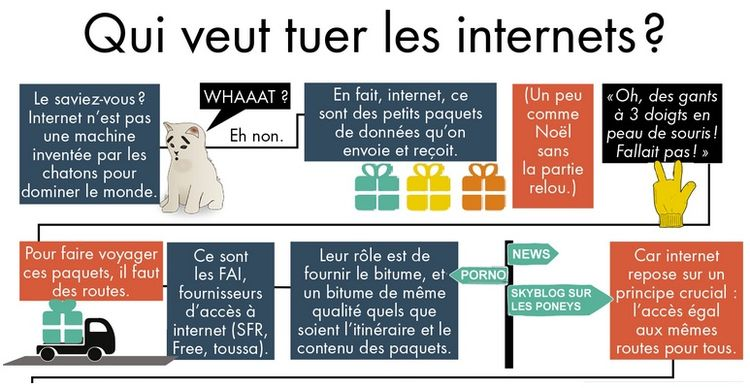
\includegraphics[width=225px]{chapters/02/images/internet_cats.jpg}
    \caption{\label{netneutrality}\emph{La neutralité du net} \cite{NetNeutrality1}.}
\end{figure}

\paragraph{} Cette forme \emph{d'inégalité} est dangereuse car elle met en péril les fondements d'internet
en en faisant une plateforme commerciale. Cela oblige certains utilisateurs à changer leur utilisation
et les invite à trouver des moyens détournés, en passant par les \emph{réseaux parallèles} par exemple, pour
parvenir à garder la même utilisation. En France, la neutralité du net à été estimée comme un droit par
le \emph{Conseil Constitutionnel}, ce qui constitue selon nous une avancée importante. En reconnaissant la
nécessité de pouvoir s'exprimer librement et d'avoir accès de manière égale aux différents contenus proposés
sur le net, le gouvernement s'inscrit dans une relation de confiance avec la population qui nous semble
nécessaire dans le contexte géopolitique actuel. Nombreux sont les pays dans lesquels l'accès à internet
est contrôlé. Gouvernement religieux, autocratique, totalitaire, militariste.. Chaque contexte implique
des restrictions différentes, mais qui portent atteinte selon nous à \emph{la liberté d'expression}.

\paragraph{Crypto-monnaies et régulation} Remarquons que le phénomène récent des \emph{crypto-monnaies}, qui
se concrétisent à travers l'utilisation de blockchains, sont particulièrement sensibles aux \emph{comportements
et annonces} des différents gouvernements vis-à-vis de cette technologie. Ainsi, courant Janvier 2018, le Bitcoin
ainsi que différentes crypto-monnaies perdaient jusqu'à plus de $20\%$ de leur valeur, suite à une annonce du 
gouvernement corréen visant à \emph{interdire l'accès aux plateformes d'échanges de crypto-monnaies} dans le pays.
\cite{CryptoMonnaies0} Quelques mois avant, Septembre 2017, c'était une annonce d'une grande plateforme chinoise
d'échange qui faisait perdre au Bitcoin $17\%$ de sa valeur en deux jours. \cite{CryptoMonnaies1}

\paragraph{} Finalement, Internet et les réseaux à grande échelle restent beaucoup contrôlés par les entités
gouvernementales et politiques. Les fournisseurs d'accès internet et les hébergeurs sont devenus deux 
nouvelles puissances actives \emph{d'établissement ou de relâchement du contrôle}. Les utilisateurs quant à eux
acceptent \emph{davantage} de contrôle et ce plus \emph{facilement} qu'auparavant. l'accès à des données personnelles
n'est pas questionné car il n'est parfois même pas \emph{conscient}.